% Uncomment this to make slides with overlays:
%\documentclass[slides]{beamer}

% Uncomment these (but comment the above \documentclass line) to make handouts:
\documentclass[handout]{beamer}

% Uncomment these to have more than one slide per page
%\usepackage{pgfpages}
%\pgfpagesuselayout{2 on 1}[border shrink=5mm]
%\pgfpageslogicalpageoptions{1}{border code=\pgfusepath{stroke}}
%\pgfpageslogicalpageoptions{2}{border code=\pgfusepath{stroke}}

\usepackage[]{graphicx, color, hyperref}

\mode<presentation>
{
	%\usetheme[secheader]{Boadilla}
	%\usecolortheme[rgb={.835, .102,.169}]{structure}  
	\usetheme[width= 0cm]{Goettingen}
	%\setbeamercovered{transparent}
}
\setbeamertemplate{navigation symbols}{}
\setbeamertemplate{footline}[frame number]

\definecolor{blue2}{rgb}{0.278,0.278,0.729} 
\newcommand{\blue}[1]{\textcolor{blue2}{#1}}
\newcommand{\white}[1]{\textcolor{white}{#1}}
\newcommand{\red}[1]{\textcolor{red}{#1}}
\newcommand{\xbar}{\overline{x}}
\newcommand{\ybar}{\overline{y}}
\newcommand{\phat}{\widehat{p}}
\newcommand{\prob}{\mbox{Pr}}
\newcommand{\E}{\mathbb{E}}
\newcommand{\Var}{\mbox{Var}}
\newcommand{\cp}{\oplus}
\newcommand{\cm}{\circleddash}

\title{Lecture 7: Probability}
\author{Chapter 2.x}
\date{}


\begin{document}
%------------------------------------------------------------------------------
\begin{frame}
\titlepage
\end{frame}
%------------------------------------------------------------------------------


%------------------------------------------------------------------------------
\begin{frame}[fragile]
\frametitle{Outcomes}
Probability forms the theoretical backbone of statistics.  We use probability to characterize randomness.  

\vspace{0.25cm}

We often frame probability in terms of a \blue{random process} giving rise to an \blue{outcome}.  

\vspace{0.25cm}

\pause Typical examples
\begin{itemize}
\item Die roll: 6 outcomes
\item Coin Flip: 2 outcomes
\end{itemize}

\end{frame}
%------------------------------------------------------------------------------


%------------------------------------------------------------------------------
\begin{frame}[fragile]
\frametitle{Disjoint AKA Mutually Exclusive Outcomes}

%
% Comment this
%
Two outcomes are \blue{disjoint (AKA mutually exclusive)} if they cannot both occur at the same time.  

\vspace{0.5cm}

\pause Die example:
\begin{itemize}
\pause\item Rolling a 1 and a 2 are disjoint.  
\pause\item Rolling a 1 and rolling ``an odd number'' are not disjoint.
\end{itemize}


\end{frame}
%------------------------------------------------------------------------------


%------------------------------------------------------------------------------
\begin{frame}[fragile]
\frametitle{Addition Rule of Probability}

%
% Comment this
%
If $A_1$ and $A_2$ are disjoint outcomes, then
\[
P(A_1 \mbox{ or } A_2) = P(A_1) + P(A_2)
\]

\vspace{0.5cm}

\pause Ex: Rolling 1 and 2 are disjoint, so:
\[
P(\mbox{rolling 1 or 2}) = P(\mbox{rolling 1}) + P(\mbox{rolling 2}) = \frac{1}{6} + \frac{1}{6}
\]


\end{frame}
%------------------------------------------------------------------------------


%------------------------------------------------------------------------------
\begin{frame}[fragile]
\frametitle{General Addition Rule of Probability}
%
% Comment this
%
If $A_1$ and $A_2$ are two outcomes (not necessarily disjoint), then
\[
P(A_1 \mbox{ or } A_2) = P(A_1) + P(A_2) - \blue{P(A_1 \mbox{ and } A_2)}
\]

Venn diagram:
\vspace{3cm}

\end{frame}
%------------------------------------------------------------------------------


%------------------------------------------------------------------------------
\begin{frame}[fragile]
\frametitle{General Addition Rule of Probability}
%
% Comment this
%
\blue{Events} are just combinations of outcomes. Ex: Deck of cards
\begin{itemize}
\item $A_1 =$ event we draw a diamond
\item $A_2 =$ event we draw a face card
\end{itemize}

\pause These two events are not disjoint, as there are 3 diamond face cards.
Venn diagram:
\vspace{3cm}

\end{frame}
%------------------------------------------------------------------------------


%------------------------------------------------------------------------------
\begin{frame}[fragile]
\frametitle{General Addition Rule of Probability}
%
% Comment this
%
\begin{eqnarray*}
P(A_1 \mbox{ or } A_2) &=& P(\mbox{diamond or a face card})\\
&=& P(\mbox{diamond}) + P(\mbox{face card}) - \\
&&P(\mbox{diamond AND face card})\\
&=& \frac{13}{52} + \frac{3 \times 4}{52} - \frac{3}{52} = \frac{22}{52} = 42.3\%
\end{eqnarray*}


\end{frame}
%------------------------------------------------------------------------------


%------------------------------------------------------------------------------
\begin{frame}
\frametitle{Sample Space and the Complement of Events}
%
% Comment this
%
A die has 6 possible outcomes.  The \blue{sample space} is the set of all possible outcomes $S = \{1, 2, \ldots, 6\}$.  

\pause \vspace{0.75cm}
Say event $A$ is the event of rolling an even number i.e $A=\{2, 4, 6\}$.  The \blue{complement of event} A is $A^c=\{1, 3, 5\}$ i.e. getting an odd number.  

\pause \vspace{0.75cm}
We have
\[
P(A) + P(A^c) = 1
\]

\end{frame}
%------------------------------------------------------------------------------


%------------------------------------------------------------------------------
\begin{frame}
\frametitle{Independence}
Two processes are \blue{independent} if knowing the outcome of one provides no useful information about the outcome of the other.  Otherwise they are dependent.

\vspace{0.5cm}
Consider:
\begin{enumerate}
\pause \item Die rolls
\pause \item You get a movie recommendation from your friend Robin, but then their significant other Sam also recommends it.  
\pause \item You compare test scores from two Grade 9 students in the same class.  Then same school.  Then same school district.  Then same city.  Then same state.
\end{enumerate}

\end{frame}
%------------------------------------------------------------------------------


%------------------------------------------------------------------------------
\begin{frame}
\frametitle{Independence}
%
% Comment this
%
We say that events $A$ and $B$ are \blue{independent} if
\[
P(A \mbox{ and } B) = P(A) \times P(B)
\]

\vspace{0.25cm}

\pause Ex: Dice rolls are independent:
\begin{eqnarray*}
P(\mbox{rolling 1 and then 6}) &=& P(\mbox{rolling 1}) \times P(\mbox{rolling 6})\\
&=& \frac{1}{6}\times\frac{1}{6} = \frac{1}{36}
\end{eqnarray*}

\end{frame}
%------------------------------------------------------------------------------


%------------------------------------------------------------------------------
\begin{frame}
\frametitle{Conditional Probability}
%
% Comment this
%

The \blue{conditional probability} of an event $A$ \blue{given} the event $B$, is defined by
\[
P(A|B) = \frac{P(A \mbox{ and } B)}{P(B)}
\]  

\end{frame}
%------------------------------------------------------------------------------


%------------------------------------------------------------------------------
\begin{frame}
\frametitle{Example}
Let's suppose I take a random sample of 100 Reed students to study their smoking habits.

\begin{center}
  \begin{tabular}{r|cc|c}
	&Smoker&Not Smoker&Total\\
	\hline
Male&19&41&60\\
Female&12&28&40\\
\hline
Total&31&69&100\\
\end{tabular}
\end{center}

\begin{small}
\begin{itemize}
\pause\item What is the probability of a randomly selected male smoking?
\[
P(S|M) = \frac{P(S \mbox{ and } M)}{P(M)} = \frac{19/100}{60/100} = \frac{19}{60}
\]
\pause\item What is the probability that a randomly selected smoker is female?
\[
P(F|S) = \frac{P(F \mbox{ and } S)}{P(S)} = \frac{12/100}{31/100} = \frac{12}{31}
\]
\end{itemize}
\end{small}

\end{frame}
%------------------------------------------------------------------------------


%------------------------------------------------------------------------------
\begin{frame}
\frametitle{Put It Together!  Independence and Conditional Prob.}
%
% Comment this
%
If $A$ and $B$ are independent events, then
\[
P(A \mbox{ and } B) = P(A)\times P(B)
\]

\pause then

\[
P(A|B) = \frac{P(A \mbox{ and } B)}{P(B)} = \frac{P(A)\times P(B)}{P(B)} = P(A)
\]  

\vspace{0.5cm}

\pause i.e. $P(A|B) = P(A)$: the event $B$ occurring has no bearing on the probability of $A$

\end{frame}
%------------------------------------------------------------------------------


%%------------------------------------------------------------------------------
%\begin{frame}[fragile]
%\frametitle{Independence Assumption}
%For almost \blue{all} the statistical tools we will use in this class, we need the assumption of independence\footnote{proven in MATH 391/392}.  The issue is when we draw samples from a population.  
%
%\vspace{0.5cm}
%\pause
%Once we've sampled someone/something, we don't typically \blue{put them back} into the pool of potential samples.\\
%i.e. we cross them off the list.  
%
%\vspace{0.5cm}
%\pause
%This is the concept from probability theory of \blue{sampling with replacement} vs \blue{sampling without replacement}. 
%
%\end{frame}
%%------------------------------------------------------------------------------
%
%
%%------------------------------------------------------------------------------
%\begin{frame}[fragile]
%\frametitle{Independence Assumption}
%
%Say we are interested in the probability of sampling Wayne and Mario.  For independence to hold we need
%\[
%P(\mbox{ Wayne \& Mario }) = P(\mbox{ Wayne }) \times P(\mbox{ Mario })
%\]
%\pause
%Compare $N=4$ \& $N=10000$ and assume we pick Mario first.  By conditional probability:
%\begin{eqnarray*}
%\pause P(\mbox{ Wayne \& Mario }) &=& P(\mbox{ Mario }) \times P(\mbox{ Wayne }|\mbox{ Mario }) \\
%\pause P(\mbox{ Wayne \& Mario }) &=& \frac{1}{4}\times\frac{1}{3} \ \pause \red{\neq} \  \frac{1}{4}\times\frac{1}{4}\\
%\pause P(\mbox{ Wayne \& Mario }) &=& \frac{1}{10000}\times\frac{1}{9999} \ \pause \red{\approx} \ \frac{1}{10000}\times\frac{1}{10000}
%\end{eqnarray*}
%
%\end{frame}
%%------------------------------------------------------------------------------
%
%
%%------------------------------------------------------------------------------
%\begin{frame}[fragile]
%\frametitle{Independence Assumption}
%
%\blue{Moral of the story}:  when sampling without replacement, as the size of the sample $n$ grows to be a larger and larger proportion of the total study population $N$, the independence assumption breaks down.  
%
%\end{frame}
%%------------------------------------------------------------------------------


%------------------------------------------------------------------------------
\begin{frame}
\frametitle{Gambler's Fallacy: Roulette}
\begin{center}
   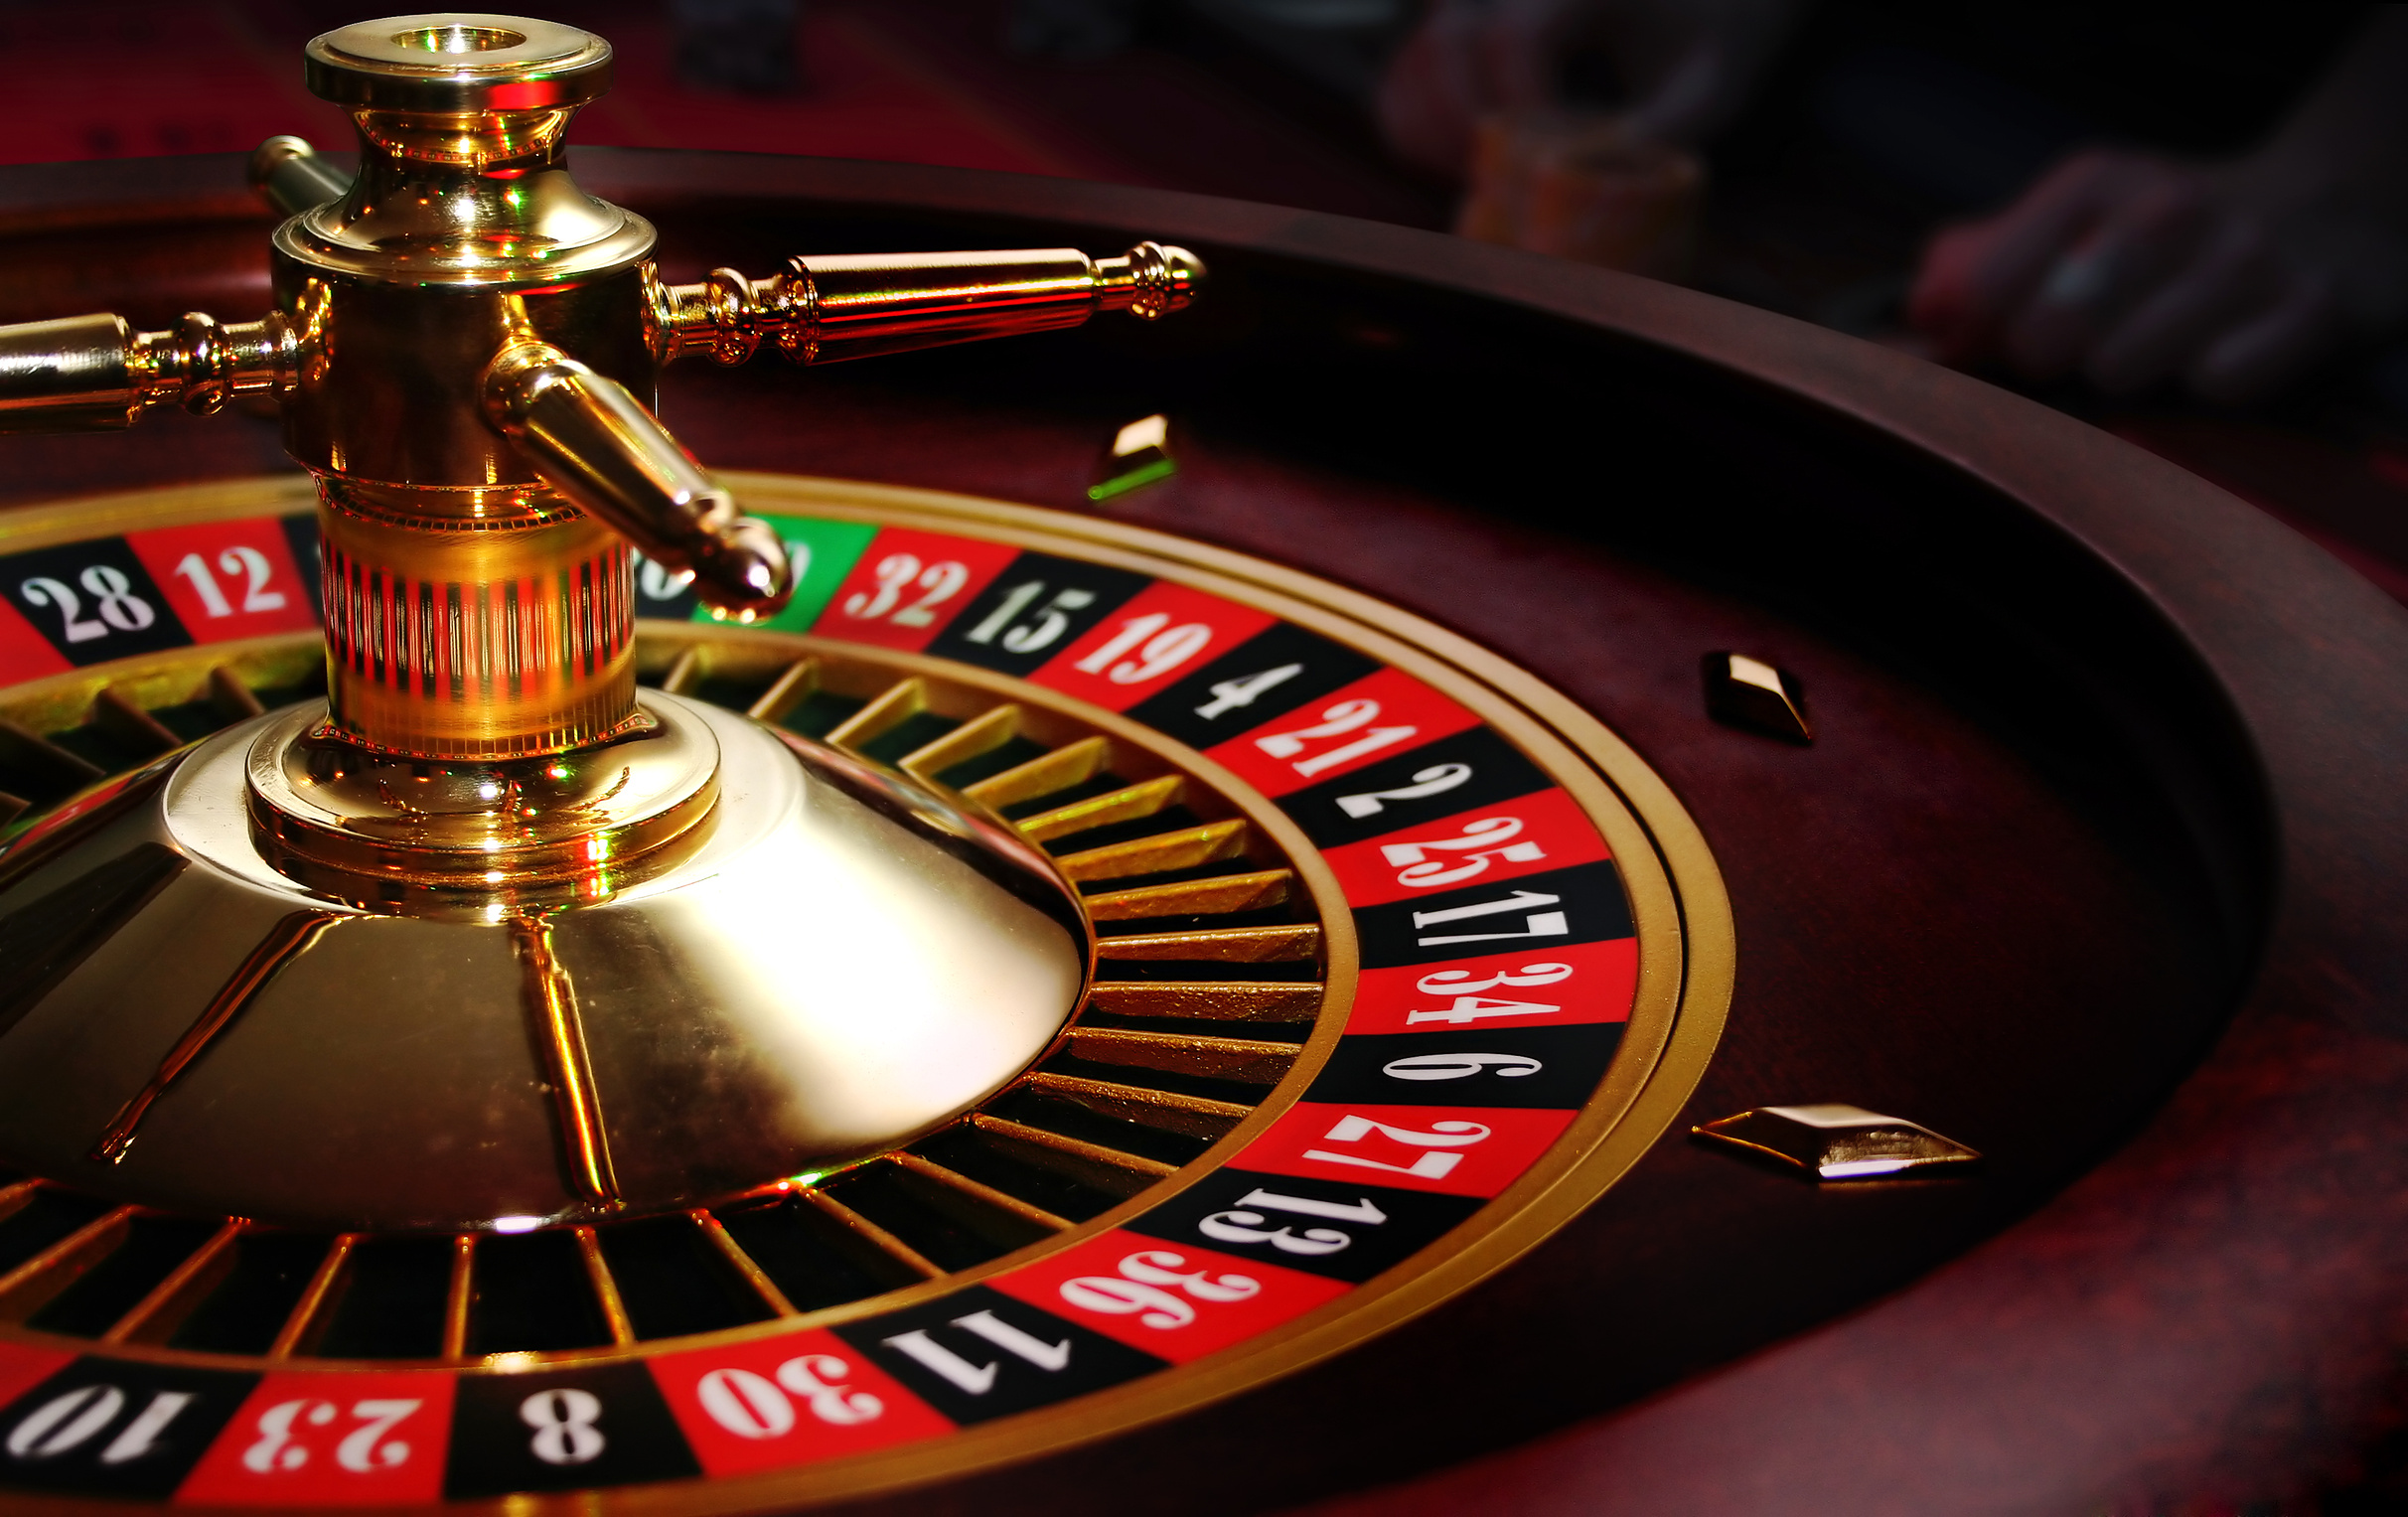
\includegraphics[width=3in]{figure/Roulette_wheel.jpg} 
\end{center}

You can bet on individual numbers, sets of numbers, or \blue{red vs black}.  Let's assume no 0 or 00, so that $P(R) = P(B) = \frac{1}{2}$.  

\end{frame}
%------------------------------------------------------------------------------


%------------------------------------------------------------------------------
\begin{frame}
\frametitle{Gambler's Fallacy: Roulette}
One of the biggest cons in casinos: \blue{spin history boards}.
\begin{center}
   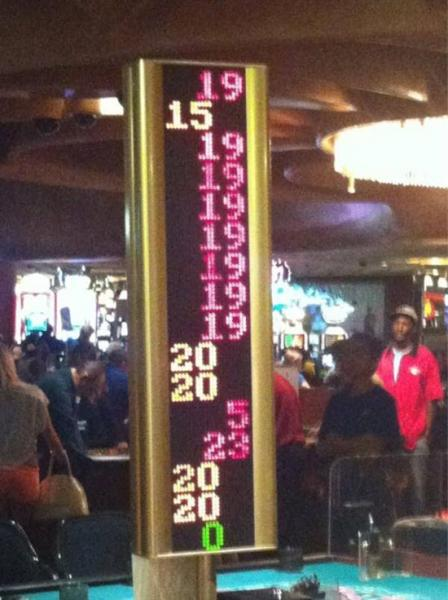
\includegraphics[height=2in]{figure/roulette.jpg} 
\end{center}
Let's ignore the numbers and just focus on what color occurred. Note: the white values on the left are \blue{black} spins.
\end{frame}
%------------------------------------------------------------------------------


%------------------------------------------------------------------------------
\begin{frame}
\frametitle{Gambler's Fallacy: Roulette}
Let's say you look at the board and see that the last 4 spins were \textcolor{red}{red}.\\

\vspace{0.25cm}

\pause You will always hear people say \blue{``Black is due!''}\\

\pause \vspace{0.25cm}

Ex. on the 5th spin people think:
\begin{eqnarray*}
P(B_5 &|& \textcolor{red}{R_1} \mbox{ and } \textcolor{red}{R_2} \mbox{ and } \textcolor{red}{R_3} \mbox{ and } \textcolor{red}{R_4}) > \\
P(\textcolor{red}{R_5} &|& \textcolor{red}{R_1} \mbox{ and } \textcolor{red}{R_2} \mbox{ and } \textcolor{red}{R_3} \mbox{ and } \textcolor{red}{R_4})
\end{eqnarray*}

\end{frame}
%------------------------------------------------------------------------------


%------------------------------------------------------------------------------
\begin{frame}
\frametitle{Gambler's Fallacy: Roulette}
But assuming the wheel is not rigged, spins are independent i.e. $P(A|B) = P(A)$.  So:

\pause \begin{eqnarray*}
P(B_5 | \textcolor{red}{R_1} \mbox{ and } \textcolor{red}{R_2} \mbox{ and } \textcolor{red}{R_3} \mbox{ and } \textcolor{red}{R_4}) = P(B_5) &=& \frac{1}{2} \\
P(\textcolor{red}{R_5} | \textcolor{red}{R_1} \mbox{ and } \textcolor{red}{R_2} \mbox{ and } \textcolor{red}{R_3} \mbox{ and } \textcolor{red}{R_4}) = P(\textcolor{red}{R_5}) &=& \frac{1}{2}
\end{eqnarray*}


\end{frame}
%------------------------------------------------------------------------------


%------------------------------------------------------------------------------
\begin{frame}[fragile]
\frametitle{Next Time}

Discuss the Normal Distribution

\begin{center}
   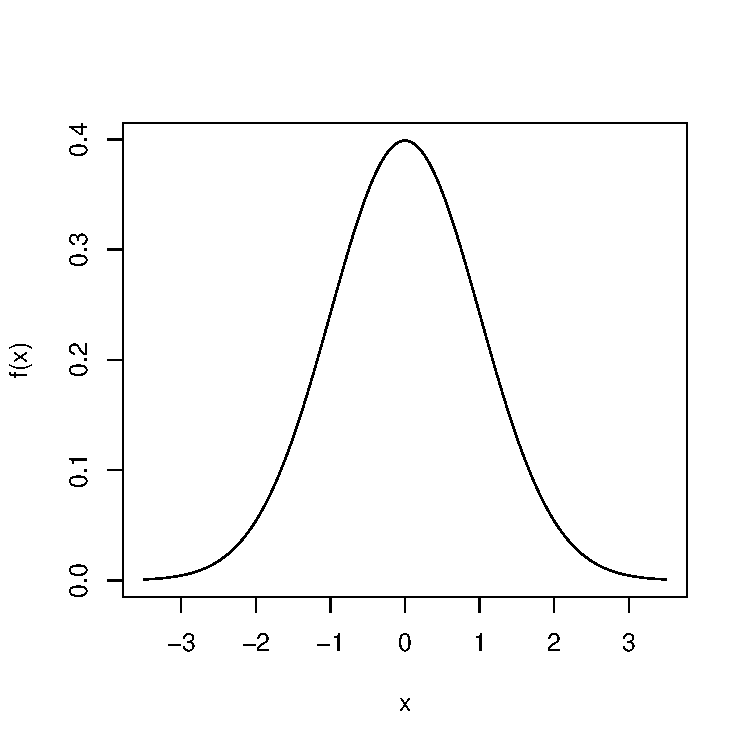
\includegraphics[width=2.5in]{figure/standard_normal.pdf} 
\end{center}

\end{frame}
%------------------------------------------------------------------------------


\end{document}










